\documentclass{BYUTextbook}

\usepackage[dutch]{babel}

\usepackage{parskip}
\usepackage{graphicx}
\usepackage{hyperref}
\usepackage{needspace}
\sloppy
%%% ---------------  onze definities ----------------

% app inventor kleuren
\definecolor{aiblue}{rgb}{0.65,.78,0.9}
\definecolor{aigreen}{rgb}{0.81,.87,0.6}

% \ai voor 'App Inventor' (ik word zo moe van steeds die hoofdletters in te moeten typen :-) )
\newcommand{\ai}[0]{\emph{App Inventor} \nolinebreak}

% gebruik \block voor een block in de AppInventor-block editor   ( voor nu: italic bold )
\newcommand{\block}[1]{\colorbox{aiblue}{ \texttt{#1} }}

\newcommand{\menuitem}[1]{\colorbox{aigreen}{ #1 }} 

\newcommand{\bestand}[1]{\url{#1}}  % eigenlijk is het gebruik van url hier niet helemaal correct omdat de link nergens naartoe wijst, maar het ziet er wel OK uit. 

% Run op telefoon
\newcommand{\runOpTelefoon}[2][0pt]{
    \marginpar{\captionsetup{type=table} \vspace{#1}
    \begin{minipage}[t][#2]{1.23in}
    \smallskip
    \footnotesize 
    \checkoddpage
    \ifoddpage
	   \RaggedRight 
    \else
	   \RaggedLeft
    \fi
    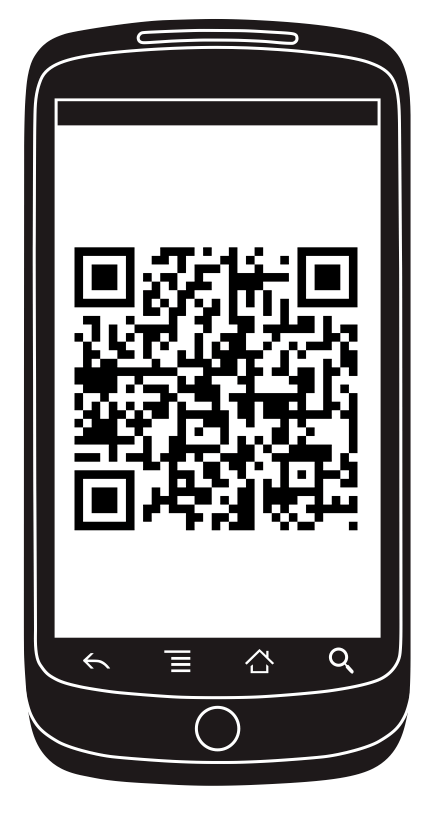
\includegraphics[width=.615in]{screenshots/run_op_telefoon}
	    
    \end{minipage}
    }
}


% Metadata, licentie
\ifpdf
\pdfinfo {
/Title (Android Apps met App Inventor)
/Author (Coen Crombach, Robin Eggenkamp, Fran\c{c}ois Vonk - CC-Licence : http://creativecommons.org/licenses/by-nc-sa/3.0/)
}
\fi

\includexmp{creativecommons}

%%% ---------------  begin van het document ----------------
\begin{document}

\frontmatter

\thispagestyle{empty}
\begin{adjustwidth}{}{-1.5in}

 \centering
 \Huge Android Apps met App Inventor
 \normalsize
 \vspace{.8in}

Coen Crombach

Robin Eggenkamp

Fran\c{c}ois Vonk

 \vspace{0.5in}

% \graphicspath{{screenshots/building_blocks/}{screenshots/AppInventorLogo/}}
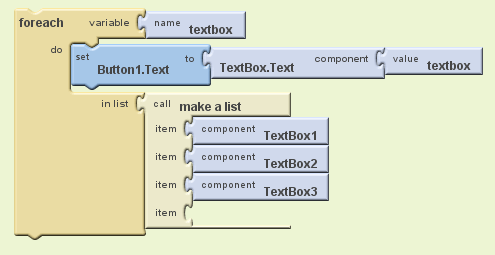
\includegraphics[width=\textwidth]{screenshots/building_blocks}

\vspace{0.25in}


\includegraphics[width=0.5\textwidth]{screenshots/AppInventorLogo}

\vspace{0.25in}

\today

\end{adjustwidth}

\newpage

\null
\vfill
\ccbyncsaeu

\small{Dit werk is gelicenseerd onder een Creative Commons Naamsvermelding-NietCommercieel-GelijkDelen 3.0 Unported. Bezoek \url{http://creativecommons.org/licenses/by-nc-sa/3.0/} om een kopie te zien van de licentie of stuur een brief naar Creative Commons, 444 Castro Street, Suite 900, Mountain View, California, 94041, USA.}

\cleardoublepage

\chapter*{Voorwoord}
\addcontentsline{toc}{chapter}{Voorwoord}

Dit boek is geschreven in het kader van Onderzoek van Onderwijs aan de Eindhoven School of Education, Technische Universiteit Eindhoven. Het boek is bedoeld voor gebruik als introductie tot programmeren in het vak Informatica in de bovenbouw van het voortgezet onderwijs. Aan de hand van enkele applicaties voor Android telefoons zul je de principes van programmeren leren.

\section*{Gebruikte notaties}
\addcontentsline{toc}{section}{Gebruikte notaties}
In dit boek worden enkele notaties gebruikt om het voor jou als lezer makkelijker leesbaar te maken. In deze sectie geven we hier een opsomming van.

\begin{description}
   \item[\block{Block}] Blocks zul je gebruiken om te programmeren. Blocks in \ai worden weergegeven als puzzelstukjes. 
   \item[\menuitem{Knop} of \menuitem{menu}] Menuopties of knoppen worden op deze manier aangegeven.
   \item[\emph{Term}] Belangrijke termen worden schuingedrukt om deze extra te benadrukken.
   \item[\lefthand\ Hints] Naast de tekst worden soms belangrijke hints of tips gegeven.
   \item[Opgaven] Opgaven worden aangeduid met een blauwe balk. 
     \begin{opgave}
       \opgVraag
	Hier staat de vraag.
       \opgUitwerking
         In sommige gevallen wordt ook een uitwerking gegeven.
     \end{opgave}
   \item[Waarschuwing] In sommige gevallen willen we je een belangrijke waarschuwing of tip geven. Deze worden voorzien van een rode balk.
     \begin{derivation}{Waarschuwing}
       Hier staat een waarschuwing, lees deze zorgvuldig!
      \end{derivation}
    \item[Uitproberen!] \runOpTelefoon{} Regelmatig kom je de afbeelding hiernaast tegen. Dit betekent dat je de app waar je op dat moment mee bezig bent uit mag proberen op je telefoon of in de emulator.
\end{description}

\tableofcontents

\mainmatter

\chapter{Installatie}

De \ai ontwikkelomgeving draait in een webbrowser. Om toegang tot \ai te krijgen heb je een Google account nodig. Je kunt zo'n account aanvragen op: \url{http://accounts.google.com/NewAccount?hl=nl} . Als je een Google account (aangemaakt) hebt kun je inloggen via de volgende link: \url{http://beta.appinventor.mit.edu}.
Nadat je ingelogd bent en een paar welkomstschermen weggeklikt hebt zie je een scherm zoals afgebeeld in figuur \ref{screenshots/projects}.

\inlinefig{screenshots/projects}{`My Projects' scherm}
 
Op school is alle software die \ai nodig heeft al voor je ge\"installeerd. Maar als je thuis aan de slag gaat is dat misschien niet zo. Daarom volgen hierna de instructies om thuis te zorgen dat de \ai ontwikkelomgeving goed werkt. Als je al een werkende omgeving hebt kun je meteen door naar het volgende hoofdstuk. 

\section{Thuis installeren}
Het is nu belangrijk dat je de software installeert die \ai nodig heeft om de \emph{Blocks Editor} en de emulator uit te voeren. Deze termen zullen je nu misschien nog niets zeggen en dat is op dit moment niet erg. Verderop in het materiaal, als je ze nodig hebt, zullen ze in detail behandeld worden. Het is nu belangrijk om op de `Learn' link te klikken, zie figuur \ref{screenshots/projects_learn}.

\inlinefig{screenshots/projects_learn}{Locatie van de `Learn' link}

Als we dit hebben gedaan zien we het scherm zoals afgebeeld in figuur \ref{screenshots/setup}. Zoals je kunt zien zijn we op dit moment ge\"interesseerd in de `Setup' link. Via deze link komen we namelijk te weten wat we allemaal moeten installeren om te kunnen werken met alle functionaliteit die \ai ons te bieden heeft.
We moedigen je echter ook aan om op de andere links te klikken en even rond te neuzen wat je daar kunt vinden. Sommige links zijn handig als je later nog eens iets op wilt zoeken.

\inlinefig{screenshots/setup}{Locatie van de `Setup' link}

Nadat je op de `Setup' link hebt geklikt, zie figuur \ref{screenshots/setup}, kom je op een pagina met installatie instructies. Voorlopig hoef je alleen `Step 1' te doen `Set up your computer', zie figuur \ref{screenshots/setup_link}.
De tweede stap mag je overslaan omdat we die in dit lesmateriaal met je gaan doorlopen.

\inlinefig{screenshots/setup_link}{Locatie van de `Set up your computer' link}

\chapter{Ontwikkelomgeving}
\label{chap:ontwikkelomgeving}

\begin{derivation}{Waarschuwing}
Voordat we van start gaan met \ai een kleine waarschuwing. De ontwikkelomgeving is niet altijd even snel en het gaat niet sneller door veelvuldig op links of knoppen te klikken. Sterker nog: dit zorgt er voor dat de omgeving nog langzamer wordt en dat er fouten op gaan treden. Om dit te voorkomen vragen we je om geduld te hebben en te wachten als de omgeving je daarom vraagt!
\end{derivation}

Als het goed is heb je het scherm voor je zoals afgebeeld in figuur \ref{screenshots/projects} en heb je nog geen projecten. Het eerste dat we daarom gaan doen is een project \emph{uploaden}. Dat wil zeggen dat we een project dat iemand anders voor ons gemaakt heeft gaan binnenhalen in de  ontwikkelomgeving. Om dit te doen klikken we op de \menuitem{More Actions}-knop en kiezen vervolgens voor \menuitem{Upload Source}, zie figuur \ref{screenshots/upload}.

\inlinefig{screenshots/upload}{Locatie van `Upload Source'} 

In ons geval gaan we het `MollenMeppen' project binnenhalen. Als we op \menuitem{Upload Source} hebben geklikt krijgen we de pop-up zoals afgebeeld in Figuur \marginfig{screenshots/upload_scherm}{`Upload Project' pop-up}\ref{screenshots/upload_scherm}. Via deze pop-up kunnen we bladeren naar de locatie van het project dat we willen binnenhalen. Vraag je docent waar je het project kunt vinden.
Als we het projectbestand hebben gevonden dan selecteren we het en klikken vervolgens op \menuitem{OK}.
 
Nadat  we op \menuitem{OK} hebben geklikt wordt het project `MollenMeppen' in ons scherm toegevoegd, zie figuur \ref{screenshots/mollenmeppen_project}.

\inlinefig{screenshots/mollenmeppen_project}{ \emph{My Projects} scherm met MollenMeppen project}

Korte tijd nadat het project is toegevoegd zal de ontwikkelomgeving automatisch naar het \emph{Design}-scherm springen waarin we het ontwerp van de applicatie zien, zie figuur \ref{screenshots/mollenmeppen_design}. Om weer naar het `My Projects' scherm te gaan kun je deze aanklikken in de ontwikkelomgeving.
\inlinefig{screenshots/mollenmeppen_design}{`Design' scherm van MollenMeppen}

\chapter{Mollen Meppen}

Je hebt zojuist je eerste project geladen en het ontwerp ervan kort gezien. Voor je het een en ander uitgebreid bekijkt ga je de applicatie eerst een keer uitvoeren.

\marginfig{screenshots/MollenMeppen_open_blocks}{Open the Blocks Editor}
Dit doe je door de \menuitem{Blocks Editor} te openen via de \menuitem{Blocks} link rechts boven in het scherm, zie figuur \ref{screenshots/MollenMeppen_open_blocks}. Nu moet je even goed opletten omdat het kan zijn dat je browser toestemming vraagt om een aantal dingen te mogen doen.

%Als eerste wordt het \bestand{AppInventorForAndroidCodeblocks.jnlp} bestand geopend. Als je browser je hierover een vraag stelt moet je op \menuitem{openen} klikken. Vervolgens wordt het bestand geladen door \emph{Java} en kan het zijn dat je toestemming moet geven om het bestand uit te voeren. 
De \menuitem{Blocks Editor} wordt geopend en je ziet wat er in figuur \ref{screenshots/MollenMeppen_BlocksEditor} is afgebeeld.

\inlinefig{screenshots/MollenMeppen_BlocksEditor}{Blocks Editor van MollenMeppen}

%\begin{derivation}{Let op}
%De \menuitem{Blocks Editor} is een aparte applicatie die niet in je webbrowser draait. Je ziet in je taakbalk dan ook een \emph{App Inventor for Android Blocks Editor: MollenMeppen - Screen1} pictogram. 
Met knoppen \menuitem{Design} en \menuitem{Blocks} (Figuur \ref{screenshots/MollenMeppen_open_blocks}) kun je wisselen tussen het \menuitem{Design} scherm en de \menuitem{Blocks Editor}.
%\end{derivation}

\marginfig{screenshots/MollenMeppen_emulator_unlock}{De emulator}
Je kunt nu met een QR-code de app op je smartphone uitproberen (Figuur \ref{screenshots/install_build_qr} een paar bladzijdes terug). 
Als je de applicatie liever wil uitvoeren in de emulator (kan alleen als die ge\"installeerd is) moet je eerst de emulator opstarten. 
\inlinefig{screenshots/MollenMeppen_Connect_menu}{Connect-menu}

\section{De emulator}
(als je met de QR-code en een Android-toestel werkt kun je door naar het volgende hoofdstuk).

Het opstarten van je app in de emulator doe je via \menuitem{Emulator} (zie Figuur \ref{screenshots/MollenMeppen_Connect_menu}).
Als de emulator is opgestart ziet deze er uit zoals afgebeeld in figuur \ref{screenshots/MollenMeppen_emulator_unlock}. De emulator staat nu nog `op slot', je kunt het slot verwijderen door met de muis op het \menuitem{slotje} te klikken, de muisknop ingedrukt te houden, de muis in de richting van de pijl te bewegen zoals aangegeven in figuur \ref{screenshots/MollenMeppen_emulator_unlock} en de muisknop weer los te laten.
\marginfig{screenshots/MollenMeppen}{MollenMeppen}

%\pagebreak
\begin{derivation}{Let op}
Zorg ervoor dat je de emulator maar \'e\'en keer opstart. Het meerdere keren opstarten van de emulator leidt tot een instabiele situatie en zorgt ervoor dat op den duur de boel kan crashen.
\end{derivation}

%\inlinefig{screenshots/MollenMeppen_BlocksEditor_New_emulator}{Locatie van de \menuitem{New emulator} link}

%Als je de emulator `van slot' hebt gehaald kun je verbinding maken met de emulator. Dit doe je door op de \menuitem{Connect to Device} link te klikken en vervolgens \menuitem{emulator-5554} te kiezen, zie figuur \ref{screenshots/MollenMeppen_BlocksEditor_Connect_to_Device}.

%\inlinefig{screenshots/MollenMeppen_BlocksEditor_Connect_to_Device}{Locatie van de \menuitem{Connect to Device} link}

Nadat je op de link geklikt hebt wordt je applicatie in de emulator geladen. 


\section{Testen (Android of emulator)}
Als het laden klaar is zie je wat er is afgebeeld in figuur \ref{screenshots/MollenMeppen} en kun je de applicatie gebruiken. Klik op de mol en kijk wat er gebeurt.
 
Wat er gebeurt is nog niet zo heel spannend en uitdagend, maar daar kun je wat aan doen! Hieronder volgt een serie opdrachten waardoor je `Mollen Meppen' tot een echt spel kunt maken. We raden je aan om na iedere opgave waarin je de code aanpast deze uit te testen op de emulator. Veel plezier en succes!

\section{Blocks Editor}
Voordat je de code gaat aanpassen staan we even stil bij het scherm wat je nu voor je hebt staan, de \menuitem{Blocks Editor}. Dit scherm gebruik je om te programmeren. Net als het \menuitem{Design} scherm bestaat ook dit scherm uit verschillende onderdelen. Deze onderdelen zie je in figuur \ref{screenshots/MollenMeppen_BlocksEditor_onderdelen}.

\inlinefig{screenshots/MollenMeppen_BlocksEditor_onderdelen}{De verschillende onderdelen van de \menuitem{Blocks Editor}}

\begin{description}
  \item[1. De knoppenbalk] In deze balk vind je knoppen om het project op te slaan, stappen ongedaan te maken en om met de emulator te communiceren.
  \item[2. Palette] Het palette is de plek waar je alle categorie\"en van \emph{blocks} vindt die je kunt gebruiken in jouw apps. Onder de tab \menuitem{My Blocks} vind je de door jouw aangemaakte componenten. Hierachter vind je de bijbehorende \emph{blocks}, hiermee kun je bijvoorbeeld een actie koppelen aan een knop.
  \item[3. Blocks] Als je in het palette een categorie aanklikt verschijnt dit overzicht. Hierin vind je de \emph{blocks} zelf die je naar het canvas kunt slepen om ze te gebruiken.
  \item[4. Canvas] In dit deel ontwerp je de gebruikersinterface van je applicatie. Vanuit het palette sleep je \emph{blocks} in het canvas. Wil je een \emph{block} verwijderen, dan sleep je deze naar de prullenbak rechtsonder.
\end{description}

%\pagebreak
\begin{derivation}{Let op}
Op het moment dat je een component in het \menuitem{Design} scherm sleept of een bestaande component een andere naam geeft, dan moet de \menuitem{Blocks Editor} automatisch bijgewerkt worden. Helaas gaat dit niet altijd goed. Als je merkt dat de \menuitem{Blocks Editor} niet meer klopt bij je \menuitem{Design} scherm, sluit de \menuitem{Blocks Editor} dan af en start hem opnieuw op.
\end{derivation}

\section{Willekeurig opduiken van de mol}
De mol beweegt zich erg voorspelbaar op dit moment en dat maakt het spel saai. In de \menuitem{Blocks Editor} kun je zien waarom de mol zich zo gedraagt.

\begin{opgave}
    \opgVraag
	Bekijk de code van de procedure `verplaatsMol' en beredeneer waarom de mol zich verplaatst 
	zoals je ziet wanneer je erop klikt. 
\end{opgave}

\begin{derivation}{Procedures}
\label{der:procedures}
Als je de code bekeken hebt zoals in de opgave hiervoor gevraagd werd, is je hopelijk opgevallen dat er een zogenaamde procedure is gemaakt met de naam `verplaatsMol'. Deze procedure wordt aangeroepen vanuit `ImageSpriteMol.Touched'.

Een procedure (ook vaak \emph{functie} of \emph{methode} genoemd) is een stuk code met een naam. In ons geval `verplaatsMol'. Via de naam kan de bijbehorende code uitgevoerd worden. De naam is als het ware een afkorting voor het stuk code.

Procedures zijn handig omdat ze voorkomen dat je hetzelfde stuk code steeds opnieuw moet maken als je die code op meerdere plaatsen nodig hebt. Dit is minder werk en beperkt tevens de lengte van je applicatie. Wanneer je bovendien duidelijke namen gebruikt is je code ook makkelijker te lezen. Dit alles draagt bij aan de overzichtelijkheid en daarmee de onderhoudbaarheid van de code.
\end{derivation}

\marginfig[-2 inch]{screenshots/MollenMeppen_BlocksEditor_Built-In_Math}{Locatie van de `Built-In' Math link}
Wat je hier feitelijk wilt is dat de $x$ en $y$ positie van de mol (de \emph{ImageSprite}) willekeurig bepaald worden. Hiervoor kun je een \emph{block} vinden onder de \menuitem{Built-In} tab bij \menuitem{Math}, zie figuur \ref{screenshots/MollenMeppen_BlocksEditor_Built-In_Math}. \emph{Blocks} uit de \menuitem{Blocks Editor} kun je simpelweg in het \menuitem{canvas} slepen en daar neerzetten of in elkaar klikken. Als je per ongeluk een verkeerd \emph{block} hebt gebruikt kun je het verwijderen door het naar de prullenbak rechts onder in het scherm te slepen en het \emph{block} los te laten.


\pagebreak
\needspace{5\baselineskip}
\reminder[+.2in]{\lefthand}{Hint: Wat is het Engelse woord voor willekeurig?}
\begin{opgave}
    \opgVraag
	Verander de code van de procedure \emph{verplaatsMol} zodat de mol zich willekeurig verplaatst binnen het veld.
\end{opgave}


\section{Geluid toevoegen als je de mol raakt}
Als de mol geraakt wordt is het leuk als je dat ook hoort. Gelukkig kun je dit programmeren in \ai. Bij het materiaal zit een bestand \emph{whack.mp3} dat je hiervoor kunt gebruiken. Als je dit bestand niet kunt vinden vraag dan aan je leraar waar het staan.

Om \emph{whack.mp3} in je project te krijgen moet je het geluidsbestand toevoegen aan de media. Dit kun je doen via het \menuitem{Design} scherm. Als je niet kunt vinden waar je moet zijn kijk dan eens terug in dit boek naar figuur \ref{screenshots/Ontwikkelomgeving_DesignEditor}.

\begin{opgave}
    \opgVraag
	Voeg het geluid toe aan het spel. 
\end{opgave}

Als je \emph{whack.mp3} hebt toegevoegd en je gaat naar de \menuitem{Blocks Editor} dan zie je dat onder de \menuitem{My Blocks} tab \menuitem{Sound1} is toegevoegd. Hieraan zijn diverse \emph{blocks} gekoppeld die met het afspelen van geluiden te maken hebben. 
 
\begin{opgave}
    \opgVraag
	Speel het toegevoegde geluid af op het moment dat de mol geraakt wordt. 
\end{opgave}


\section{De mol op een timer laten bewegen}
Op het moment is het zo dat de mol zich alleen verplaatst als je hem een mep verkoopt. Het is leuker als de mol af en toe uit zichzelf ergens anders opduikt. Om dit voor elkaar te krijgen ga je een zogenaamde \menuitem{timer} gebruiken.
 
\marginfig{screenshots/MollenMeppen_design_clock1}{Locatie van de \menuitem{Clock} component in het palette}
Een timer kun je vinden via de \menuitem{Clock} component in het \menuitem{Sensors} palette, zie figuur \ref{screenshots/MollenMeppen_design_clock1}. 
Een component kun je in het \menuitem{Viewer} gedeelte van je ontwikkelomgeving slepen. Je ziet dat de component ook toegevoegd wordt in het \menuitem{Components} gedeelte van je ontwikkelomgeving. Dit is de plaats waar je componenten een andere naam kunt geven en verwijderen.
 
 
\begin{opgave}
    \opgVraag
	Voeg een \menuitem{Clock} component aan het spel toe en kijk goed waar deze neergezet wordt. Staat daar ook nog een andere component?

  Beredeneer waarom de clock en de andere component hier neergezet worden. 
\end{opgave}

Nadat je de \menuitem{Clock} component hebt toegevoegd kun je de timer programmeren. Hiervoor moet je in de \menuitem{Blocks Editor} zijn. 
Onder de \menuitem{`Screen1'} (linkerzijde) staat nu een \menuitem{Clock1} link omdat je de \menuitem{Clock} component hebt toegevoegd, zie figuur \ref{screenshots/MollenMeppen_design_clock1}. Klik op de link en je ziet bovenaan een \block{Clock1.Timer} block.

%\inlinefig{screenshots/MollenMeppen_BlocksEditor_Clock1}{Locatie van de \menuitem{My Blocks} | \menuitem{Clock1} link}
 
%\reminder{\lefthand}{Hint: Kijk eens bij de \menuitem{My Blocks} | \menuitem{My Definitions} link.}
\begin{opgave}
    \opgVraag
	Voeg het timer blok toe en zorg dat de mol zich om de zoveel tijd uit zichzelf verplaatst.
\end{opgave}

Als je niet weet hoe een timer werkt of je komt er niet helemaal uit, klik dan eens op de `Learn' link in je \menuitem{Design} scherm. Je kunt dan bij de \emph{Reference Documentation} op zoek gaan naar hoe een timer werkt.

Hopelijk valt je op dat de documentatie net zo is opgezet als de ontwikkelomgeving van \ai zelf. Er wordt onderscheid gemaakt tussen componenten (dingen uit je \menuitem{Design} scherm) en blocks (dingen uit de \menuitem{Blocks Editor}).

Kijk eens goed in je \menuitem{Design} scherm waar de \menuitem{Clock} component zit en ga dan in de documentatie zoeken.

\begin{derivation}{Procedures}
Als het goed is heb je nu voordeel gehad van de procedure die we al voor je gemaakt hebben. In plaats van de code opnieuw te maken heb je als het goed is nu de procedure aangeroepen.
\end{derivation}


\section{Tellen van het aantal maal dat je mis slaat}
Naast het bijhouden hoe vaak een speler de mol raakt wil je ook graag bijhouden hoe vaak de speler mis slaat. In je \menuitem{Components} staat een \block{HorizontalArrangementGeraakt} die ervoor zorgt dat je componenten horizontaal in je scherm kunt rangschikken. De componenten erin (\block{LabelGeraaktTekst} en \block{LabelGeraaktTeller}) komen overeen met `aantal geraakt' en `0' in je \menuitem{Viewer}.

\begin{derivation}{Let op}
Een label gebruik je om een stuk tekst weer te geven.
Een TextBox gebruik je om de gebruiker iets in te laten voeren.
\end{derivation}

\reminder{\lefthand}{Hint: Op het moment dat je de mol raakt gaan er twee events af namelijk `CanvasMollenVeld.Touched' en `ImageSpriteMol.Touched'. Hoe kun je deze slim gebruiken om te bepalen wanneer je mis slaat?}
\begin{opgave}
    \opgVraag
	Breid de bestaande interface uit met een \block{HorizontalArrangement} dat daarin labels heeft voor `aantal gemist' en de bijbehorende teller. Breid bovendien je programma in de \menuitem{Blocks Editor} uit zodat het aantal keer dat de speler misslaat wordt bijgehouden. 
\end{opgave}


\section{Score toevoegen}
Het bijhouden van het aantal keer raak en mis slaan is leuk maar een score is nog leuker. Voor iedere keer dat een speler de mol raakt krijgt hij/zij 2 punten. Voor iedere keer dat de speler de mol mist verliest hij/zij een punt. 

\begin{opgave}
    \opgVraag
	Voeg een \menuitem{HorizontalArrangement} toe in de \menuitem{Viewer} waarin je de score informatie laat zien. Breid bovendien je programma in de \menuitem{Blocks Editor} uit zodat de score wordt bijgehouden. 
\end{opgave}


\section{De mol sneller laten bewegen bij hoge score}
Naarmate de tijd vordert, en hopelijk de score hoger wordt, blijft de uitdaging van het spel op dit moment gelijk. Het spel vereist dus helaas niet steeds meer van het reactievermogen van de speler maar dat kun je veranderen.

Daarvoor moet je onder bepaalde voorwaarden de mol steeds sneller laten bewegen. Om dit voor elkaar te krijgen heb je een zogenaamd \emph{if-statement} nodig. Zo'n \emph{if-statement} kun je vinden in de \menuitem{Blocks Editor} in de tab \menuitem{Built-In} onder \menuitem{Control}. Daar vindt je de \block{if} en \block{ifelse} \emph{blocks}.

Bij een \emph{if-statement} wordt er getest of een expressie waar of niet waar is (we noemen zo'n expressie een \emph{Booleaanse expressie}). Als de expressie waar is wordt de code die binnen het \emph{if-statement} staat wel uitgevoerd en anders wordt deze code overgeslagen.

%\needspace{5\baselineskip}
\reminder[-1in]{\lefthand}{Hint: Als je de \menuitem{Clock} component selecteert in bijvoorbeeld de \menuitem{viewer} zie je bij \menuitem{Properties} een veld dat \emph{TimerInterval} heet. Kun je iets vergelijkbaars vinden in de \menuitem{Blocks Editor}?}
\begin{opgave}
    \opgVraag
	Zorg ervoor dat voor elke 50 punten die de speler heeft de mol 50 milliseconden sneller beweegt. Houd rekening met een grens voor de snelheid.
\end{opgave}

\begin{derivation}{Conditioneel uitvoeren van code}
Het conditioneel uitvoeren van code gebeurt bij het programmeren vaak met \emph{if-statements}. Er zijn echter ook nog andere manieren zoals bij \ai het \block{choose} \emph{block}.

\emph{if-statements} zijn belangrijk en essentieel bij het programmeren. Ze zorgen ervoor dat delen van het programma alleen onder bepaalde voorwaarden worden uitgevoerd.

We noemen dit program control en het geeft gebruikers van onze applicatie de mogelijk om de flow van het programma te be\"invloeden.
\end{derivation}


\section{Testen op je telefoon}
\runOpTelefoon{} Test de app nog eens. Als je de app op je eigen telefoon probeert, kun je hem thuis en aan vrienden laten zien!

%Vanuit de design omgeving kun je rechtsboven kiezen voor \menuitem{Package for Phone} en vervolgens \menuitem{Show barcode}. Na verloop van tijd (afhankelijk van de drukte kan dit enkele minuten duren) krijg je een venster met daarin een zogenaamde QR-code. Deze code kun je scannen met de camera van je telefoon. Hiervoor heb je een app nodig, een voorbeeld is \emph{Qr Barcode Scanner}, je kunt deze downloaden in de \emph{Play Store}.

%Na het openen van Qr Barcode Scanner kies je voor \menuitem{Scan Barcode}, je kijkt nu door je camera. Richt de camera op de barcode op het scherm. De app leest de barcode en geeft je de optie de URL die hierin verstopt is te openen in de browser. Na het openen van de browser wordt de download van een .apk bestand gestart. 

%Na het downloaden open je het bestand. Wat er precies gebeurt is afhankelijk van je telefoon en de versie van Android. Waarschijnlijk krijg je eerst de melding dat de installatie is geblokkeerd. Android telefoons zijn standaard ingesteld dat ze enkel applicaties vanuit de Market of Play Store kunnen installeren. Door \menuitem{Onbekende bronnen} aan te vinken in het \menuitem{Beveiliging} onderdeel van \menuitem{Instellingen} kun je dit toestaan. Nadat je dit hebt gedaan open je de .apk opnieuw. Je krijgt nu de vraag of je de applicatie wilt installeren, je kiest voor de knop \menuitem{Installeren}. Na enkele ogenblikken is de applicatie ge\"installeerd en kun je deze \menuitem{Openen}. 

De volgende keer dat je de applicatie via een barcode wilt installeren zal de telefoon vragen of je de applicatie wilt vervangen, dit bevestig je door op \menuitem{OK} te klikken en de applicatie vervolgens op dezelfde manier te \menuitem{Installeren}.


\pagebreak
\section{Bonus opgaven}
\reminder[+.2in]{\lefthand}{Tip: Kijk eens bij `Properties' van de \block{canvas} component.}
\begin{opgave}
    \opgVraag
  De achtergrond van het spel is op het moment saai wit.
  Voeg een achtergrond toe aan het spel om de boel wat op te fleuren.
\end{opgave}

\begin{opgave}
    \opgVraag
  Je kunt op dit moment nog niet afgaan bij het spel.
  Verander dit door de speler af te laten gaan wanneer zijn/haar score onder de 0 punten zakt.
\end{opgave}

Het afgaan in het spel kun je ook op een heel andere manier aanpakken. Je kunt de speler bij het begin van het spel een aantal levens geven en onder bepaalde omstandigheden laten verliezen. De speler is af wanneer hij/zij geen levens meer over heeft.

\reminder[+.2in]{\lefthand}{Tip: Laat het andere dier vaker verschijnen naarmate de speler een hogere score bereikt.}
\begin{opgave}
    \opgVraag
  Bouw het concept van levens in je spel in. Om levens te verliezen voeg je nog een ander dier toe aan het spel, bijvoorbeeld een lief konijntje of juist een gruwelijk monster. Laat het andere dier af en toe verschijnen in plaats van de mol en wanneer de speler het andere dier mept verliest hij/zij een leven.
\end{opgave}

\chapter{Schrandere Scholier}

In het vorige hoofdstuk heb je een leuk spel gemaakt, je kunt echter ook serieuze applicaties schrijven. Waarschijnlijk vraag je jezelf wel eens af welk cijfer je moet halen voor een toets om een 8 gemiddeld te blijven staan voor een vak. In dit hoofdstuk ga je hier een hulpmiddel voor ontwikkelen.

Je zult de applicatie stap-voor-stap opbouwen. Je maakt een begin met de gebruikersinterface in het \menuitem{design} scherm. Daarna zul je in de \menuitem{Blocks}-editor ervoor zorgen dat de gebruiker cijfers kan invoeren waarmee je vervolgens kunnen gaat rekenen. Tot slot zorg je ervoor dat de gegevens opgeslagen worden zodat je niet bij elke start opnieuw hoeft te beginnen.

\section{Een nieuw project aanmaken}
Je begint met het aanmaken van een nieuw project. In hoofdstuk \ref{chap:ontwikkelomgeving} heb je een project aangemaakt door een bestaand project te uploaden. Dit keer begin je vanaf het begin. 

Als je nog niet in het \menuitem{My Projects} scherm bent, ga hier dan nu naar toe. Klik op de knop \emph{new} om het venster zoals is weergegeven in figuur \marginfig{screenshots/SchrandereScholier_new_scherm}{`New App Inventor for Android Project'\ pop-up}\ref{screenshots/SchrandereScholier_new_scherm} te zien. Vul hier de naam van het project in, in dit geval `SchrandereScholier'. Na een klik op \menuitem{OK} wordt je nieuwe project aangemaakt en kom je terecht in het \menuitem{design}-scherm.

\section{Gebruikersinterface}
Na het aanmaken van het project begin je met het ontwerpen van de gebruikersinterface. Voordat je hiermee aan de slag gaat: bekijk de verschillende onderdelen van het scherm nog eens in hoofdstuk \ref{sec:design-scherm}.

Nu je een idee hebt van de interface kunnen we deze gaan gebruiken. Je begint eenvoudig met het toevoegen van enkele \block{labels}, \block{TextBoxen} en een \block{knop}. \reminder{\lefthand}{Een label gebruik je om een stukje tekst weer te geven.}\marginfig{screenshots/SchrandereScholier_label}{Label}Sleep hiervoor eerst een \block{Label} vanuit het \menuitem{Palette} naar de \menuitem{Viewer}. Componenten worden automatisch uitgelijnd, het \block{label} komt daardoor linksboven te staan. Pas nu de tekst van het zojuist aangemaakte \block{Label} aan in het \menuitem{Properties} paneel naar `Toets 1'. Om onze applicatie overzichtelijk te houden pas je ook de naam van het component aan. Hiervoor selecteer je het label in het \menuitem{Components} paneel en gebruik je de knop \menuitem{Rename} om het label te hernoemen naar `Toets1Label'.
\reminder{\lefthand}{Geef componenten altijd een duidelijke naam, dit maakt het programmeren makkelijker!}
Om te zorgen dat er ook cijfers ingevoerd kunnen worden voeg je een \block{TextBox} toe. 
Sleep dus een \block{TextBox} naar de \menuitem{Viewer}. Geef de \block{TextBox} de naam `Toets1'. 

\begin{opgave}
    \opgVraag
	Herhaal deze handelingen totdat je drie toetsen kunt invoeren.
\end{opgave}

Zodra de gebruiker de cijfers heeft ingevoerd zul je het cijfer moeten uitrekenen wat de gebruiker moet halen voor de volgende toets om een 8 gemiddeld te halen. De berekening doe je later, maar je voegt nu al wel een knop en twee labels toe om het resultaat weer te geven. Een knop voeg je toe door een \block{Button} vanuit het Palette naar de Viewer te slepen. Net als bij een label kun je een text opgeven in het \menuitem{Properties} paneel, vul hier `Bereken' in. Geef de \block{Button} vervolgens de naam `Bereken'.

\begin{opgave}
    \opgVraag
Maak nu de gebruikersinterface verder af, zodat deze er hetzelfde uit ziet als in figuur \ref{screenshots/SchrandereScholier_ontwerp1}.
\inlinefig{screenshots/SchrandereScholier_ontwerp1}{Gebruikersinterface van de Schrandere Scholier}
\end{opgave}

\runOpTelefoon{}
Je hebt nu de gebruikersinterface gemaakt, je kunt de applicatie nu dus al uitproberen op je telefoon of in de emulator! Je zult zien dat je al cijfers kunt invoeren, er gebeurt echter nog niks als je op de knop drukt. Daar ga je nu iets aan doen!

\section{Rekenen}
Je gaat nu zorgen dat de applicatie daadwerkelijk kan rekenen. Hiervoor moet je programmeren en dit doe je in de \menuitem{Blocks Editor}. Deze open je via de knop \menuitem{Open the Blocks Editor} rechtsboven aan. \reminder{\lefthand}{Een uitgebreidere uitleg vind je in hoofdstuk \ref{chap:ontwikkelomgeving}} Het scherm is nog helemaal leeg. Aan de linker kant staan de verschillende ingebouwde codeblokken, opgedeeld in verschillende categorie\"en, die je kunt gebruiken. \marginfig{screenshots/SchrandereScholier_my_blocks}{My Blocks van de Schrandere Scholier}Naast de ingebouwde codeblocks zijn er ook blocks speciaal voor jouw applicatie, deze vind je onder \menuitem{My Blocks}. Voor elk component dat je hebt aangemaakt in de gebruikersinterface kun je hier codeblocks vinden.

Je wilt dat er gerekend gaat worden zodra er op de knop Bereken geklikt wordt. Hier is een speciaal block voor, genaamd \block{Bereken.Click}. Je gebruikt dit block door eerst op Bereken te klikken en vervolgens \block{Bereken.Click} naar rechts te slepen. Alle codeblocks die je in dit block hangt worden uitgevoerd als er op de knop geklikt wordt.

Je begint met het verzamelen van de gegevens waarmee je straks kunt rekenen. De cijfers moet je uitlezen uit de \block{TextBoxen}, ook hiervoor staan er blokken klaar onder \menuitem{My Blocks}. Het block \block{Toets1.Text} geeft je de inhoud van Toets1 terug. Sleep deze naar rechts om het te gebruiken. \reminder{\lefthand}{Blocks in App Inventor passen enkel op elkaar als de aansluitingen compatibel zijn. Dit is net als bij puzzelstukjes.}Zoals je waarschijnlijk ziet kun je nog niks met dit blok, de aansluiting komt namelijk niet overeen met de beschikbare aansluiting van \block{Bereken.Click}. Je hebt dus nog andere blocks nodig.

Je wilt straks kunnen rekenen, een logische plek om naar een passend block te zoeken is dus de categorie \menuitem{Math}. Sleep bijvoorbeeld het optel block naar rechts. Je zult zien dat je hier \block{Toets1.Text} in kunt hangen. Niet al deze blocks hebben dezelfde aansluiting. Hoe komt dit? Deze aansluiting betekent dat het block een bepaalde waarde (bijvoorbeeld een tekst of getal, maar ook de uitkomst van een som) vertegenwoordigt, dit noem je een \emph{expressie}. In \block{Bereken.Click} passen enkel blocks die een actie vertegenwoordigen, dit wordt ook wel een \emph{statement} genoemd. 

\begin{opgave}
    \opgVraag
Na het rekenen zul je de uitkomst in \block{TeBehalen} moeten plaatsen. Zoek nu een block op waarmee je de uitkomst van een expressie in \block{TeBehalen} kunt zetten. Voeg dit block toe aan \block{Bereken.Click}. De expressie die weergegeven moet worden is de som van \block{Toets1} en \block{Toets2}. 
    \opgUitwerking
    Het programma zou er nu uit moeten zien zoals in figuur \ref{screenshots/SchrandereScholier_bereken_click}.
    \inlinefig{screenshots/SchrandereScholier_bereken_click}{Uitwerking}
\end{opgave}

\runOpTelefoon{} Voordat je verder gaat: probeer uit of het programma werkt zoals je verwacht. Als het werkt dan wordt het tijd om jouw programma uit te breiden. Er vanuit gaande dat alle cijfers dezelfde weging hebben, hoe kun je dan eenvoudig het cijfer berekenen dat de gebruiker nodig heeft om een 8 te staan? De som van alle vier cijfers moet samen minimaal $8*4=32$ zijn. Het benodigde cijfer is dus gelijk aan 32 min het totaal van de al behaalde punten. Iemand heeft bijvoorbeeld een $9$ en tweemaal een $7$ gehaald. Dit is in totaal $9+7+7=23$. Het in dit geval te behalen cijfer is dus $32-23=9$.
 
 \begin{opgave}
    \opgVraag
Implementeer de bovenstaande berekening en zet het antwoord in \block{TeBehalen}. Je hebt hiervoor, naast de al bekende blocks, ook het aftrek-block nodig en een constant getal. Een constant getal geef je aan met het block in figuur \marginfig{screenshots/SchrandereScholier_constant_getal}{Constant getal} \ref{screenshots/SchrandereScholier_constant_getal}. 

Je moet verschillende blocks `in elkaar hangen', dit wordt \emph{nesten} genoemd. Bij het uitrekenen kijkt de computer welke gegevens hij nodig heeft om het block uit te kunnen rekenen, deze gegevens zal hij eerst opzoeken of berekenen. Zodra de computer alle gegevens heeft om een block uit te rekenen doet hij dit. In het voorbeeld van een optel-block zal hij dus eerst bepalen welke twee getallen opgeteld moeten worden, om deze vervolgens op te tellen en door te geven.
    \opgUitwerking
    Het programma zou er nu uit moeten zien zoals in figuur \ref{screenshots/SchrandereScholier_bereken_cijfer}.
    \inlinefig{screenshots/SchrandereScholier_bereken_cijfer}{Uitwerking}
\end{opgave}

\runOpTelefoon{}
Als je dit programma uitprobeert met een aantal combinaties van cijfers zullen je merken dat het nog niet optimaal werkt. Maar het werkt, en dat met maar enkele blocks! In de volgende paragraaf zul je deze applicaties verder gaan uitwerken. Je zult daarbij meer zelfstandig aan de slag gaan met \ai.

\section{Verbeteren}
De eerste verbetering die je gaat doorvoeren is het toevoegen van meer cijfers, waarschijnlijk heb je geen enkel vak waarbij je maar vier toetsen krijgt. 

 \begin{opgave}
    \opgVraag
Zorg ervoor dat er vier cijfers kunnen worden ingevoerd, waarna het vijfde cijfer wordt berekend. Noteer op welke plaatsen je een aanpassing hebt moeten maken.
\end{opgave}

Als het goed is weet je nu precies welke wijzigingen je moet maken om een nieuwe toets te voegen. Zou je dit kunnen automatiseren? Dan kun je de gebruiker zelf toetsen laten toevoegen. Uiteraard is dit mogelijk! De makkelijkste oplossing zou zijn om de gebruiker nieuwe velden te laten toe voegen, dit is echter niet mogelijk in \ai. Om dit probleem toch te kunnen oplossen heeft \ai de mogelijkheid van lijsten. Je kunt het probleem nu implementeren door gebruik te maken van \'e\'en \block{TextBox} om cijfers toe te voegen aan de lijst. Deze lijst kan vervolgens worden weergegeven en gebruikt om te rekenen. Dit ga je in deze sectie implementeren.

Allereerst maak je in de \menuitem{Blocks Editor} de lijst aan. \marginfig[-.5in]{screenshots/SchrandereScholier_makeAList}{make a list block}Je doet dit door het \block{make a list} block (uit het \menuitem{Lists} palette) het werkblad op te slepen. Zoals je ziet kun je in dit block items toevoegen, dit kan bijvoorbeeld een \block{number} zijn. Een voorbeeld zie je in figuur \ref{screenshots/SchrandereScholier_makeAList}.

\marginfig{screenshots/SchrandereScholier_variabeleLijst}{De lijst in een variabele}Om de lijst te kunnen gebruiken in de rest van de code plaats je de lijst in een \emph{variabele}. Hiermee geef je de lijst een naam zodat je hier vanuit andere blocks naar kunnen verwijzen. Je maakt een variabele aan via het \block{def} block in de categorie \menuitem{definitions} zoals je kunt zien in figuur \ref{screenshots/SchrandereScholier_variabeleLijst}. 

 \begin{opgave}
    \opgVraag
De interface kun je nu aanpassen. Maak de interface zoals is weergegeven in figuur \ref{screenshots/SchrandereScholier_ontwerp2}. Er staan twee labels in het ontwerp waarvan je later de tekst gaat aanpassen vanuit de \menuitem{Blocks editor}. Denk ook nu aan een duidelijke naamgeving van de componenten.
\inlinefig{screenshots/SchrandereScholier_ontwerp2}{Nieuwe gebruikersinterface}
\end{opgave}

Ga nu weer naar de \menuitem{Blocks editor}. Als je de knop enkel hebt hernoemd heb je hier nog een block \block{Toevoegen.Click} staan. Indien dit niet het geval is voeg je deze toe vanuit \menuitem{My Blocks}. In deze procedure moet je het nieuw ingevoerde cijfer toevoegen aan de lijst. Een item toevoegen aan de lijst kun je doen via \block{add items to list} in het \menuitem{Lists} palette. Dit block heeft twee blocks nodig als parameter, namelijk een list en een nieuw item. Bij list voeg je het \block{def} block toe welke je kunt vinden bij \menuitem{My definitions} binnen het \menuitem{My Blocks} palette, bij item voeg je een block \block{Cijfer.Text} toe. 

Om nu de ingevoerde cijfers weer te geven op de daarvoor bedoelde plaats moet je een nieuw soort block gebruiken, de \block{foreach}. Deze \emph{loop} gaat alle items uit een list langs en voert voor elk van deze items een actie uit. In dit geval kun je dit gebruiken om de cijfers in de list allemaal onder elkaar te zetten. Hoe je dit doet zie je in figuur \ref{screenshots/SchrandereScholier_toevoegen_click}.

\reminder[.2in]{\lefthand}{Weet je wat de \textbackslash n betekent in deze implementatie?}
 \begin{opgave}
    \opgVraag
Implementeer het \block{Toevoegen.Click} block zoals is aangegeven in figuur \ref{screenshots/SchrandereScholier_toevoegen_click} en probeer te doorgronden hoe dit werkt.
\inlinefig{screenshots/SchrandereScholier_toevoegen_click}{Implementatie Toevoegen.Click}
\end{opgave}

\runOpTelefoon{} Probeer de app nu uit op je telefoon of in de simulator en controleer of je de code goed hebt begrepen.

\section{Weer rekenen}
De oude methode om het benodigde cijfer te berekenen werkt nu niet meer, daar moet je iets aan doen. Omdat alle cijfers in een lijst staan moet je hier weer een \block{loop} block voor gebruiken. Om te voorkomen dat de code onoverzichtelijk wordt zul je de berekening in een aparte \emph{procedure} laten plaatsvinden. 

\begin{derivation}{Procedures met resultaat}
Op pagina \pageref{der:procedures} staat uitgelegd wat een procedure is. In het kort is een procedure een groepje statements die worden uitgevoerd als je de procedure aanroept. Op deze manier kun je statements die bij elkaar horen groeperen. Een procedure kan ook een resultaat teruggeven. Dit pas je toe om bijvoorbeeld een berekening die je meerdere malen uitvoert maar eenmalig te hoeven op te schrijven. 

Ook kan het handig zijn om een procedure te gebruiken om je code leesbaarder te maken. Een lang stuk code kun je zo opdelen in kleine, begrijpelijke stukjes code. Zorg er altijd voor dat je de procedure een betekenisvolle naam geeft.
\end{derivation}

Een nieuwe procedure met resultaat kun je aanmaken door het \marginfig{screenshots/SchrandereScholier_procedureWithResult}{procedureWithResult block}\block{procedureWithResult} block, te vinden in het \menuitem{Definition} palette, naar het canvas te slepen. Je kunt er op drie plekken blocks aanhangen. Allereerst bij `arg', hier kun je een argument meegeven aan de procedure, dit zul je hier nog niet gebruiken. Bij `do' voeg je de acties toe die moeten gebeuren. Bij return geef je een waarde die wordt teruggegeven nadat deze procedure is uitgevoerd, in ons geval zal dit het te behalen cijfer zijn.

In het `do' gedeelte van de procedure kun je hetzelfde \block{foreach} block gebruiken als in \block{Toevoegen.Click}. De naam van de variabele zul je wel aan moeten passen, aangezien elke naam maar eenmaal gebruikt mag worden. 

Je begint met het optellen van alle resultaten. Dit kun je doen op een vergelijkbare manier als het aan elkaar plakken van de teksten, zoals je dat gedaan hebt in figuur \ref{screenshots/SchrandereScholier_toevoegen_click}. Je gebruikt nu echter hetzelfde \block{+} block als je eerder gebruikt hebt. \marginfig{screenshots/SchrandereScholier_som}{som variabele}Het tussenresultaat sla je op in een nieuw aan te maken variabele zoals is te zien in figuur \ref{screenshots/SchrandereScholier_som}. Ook voor het eindresultaat maak je een variabele aan genaamd \block{teBehalen}. Gebruikmakend van de som kun je nu als volgt het te behalen cijfer berekenen: \\$(aantalOpgegevenCijfers+1) * 8 - som$ \\Het resultaat van deze berekening moet je teruggeven door het block \block{teBehalen} aan `result' te hangen.

\needspace{4\baselineskip}
 \begin{opgave}
    \opgVraag
Implementeer de procedure voor het berekenen van het te behalen cijfer volgens de bovenstaande beschrijving.
    \opgUitwerking
    Als het goed is ziet de procedure er nu uit zoals in figuur \ref{screenshots/SchrandereScholier_berekenTeBehalen} is getoond.
\end{opgave}

\begin{figure}
    \inneralign{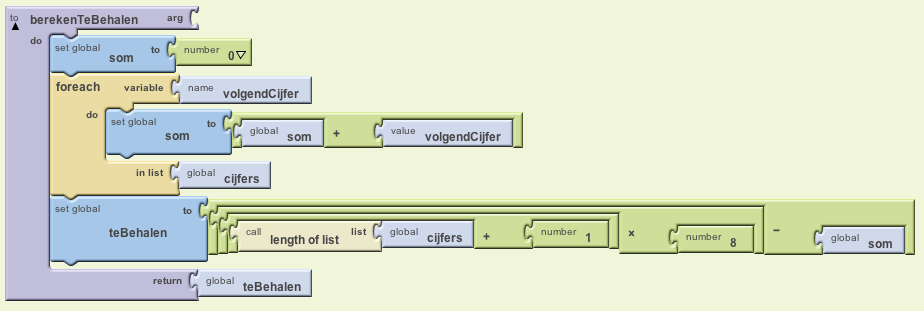
\includegraphics[width=1.4\textwidth]{screenshots/SchrandereScholier_berekenTeBehalen}}
    \caption{\label{screenshots/SchrandereScholier_berekenTeBehalen} Implementatie van berekenTeBehalen}
\end{figure}

De laatste stap is nu een klein stukje toevoegen zodat het te behalen cijfer wordt weergegeven. \marginfig{screenshots/SchrandereScholier_procedureAanroep}{Aanroepen van de bereken procedure}Dit doe je met de blocks in figuur \ref{screenshots/SchrandereScholier_procedureAanroep}. \runOpTelefoon{} 

\begin{opgave}
    \opgVraag
Voeg de blocks om het te behalen cijfer weer te geven toe aan \block{Toevoegen.Click} en test de app uit!
\end{opgave}

\begin{derivation}{Tip}
Wellicht valt je op dat er ook cijfers in de lijst staan die je niet via de app hebt ingevoerd? Als dit zo is dan heb je in de Blocks Editor nog invulling staan bij het aanmaken van de lijst. Haal deze weg en probeer het opnieuw!
\end{derivation}

\begin{opgave}
    \opgVraag
De implementatie van de procedure \block{berekenTeBehalen} is al behoorlijk ingewikkeld! Probeer de code leesbaarder te maken door de procedure op te delen in enkele korte procedures. Denk steeds goed na over welke statements je opneemt en welke naam je aan de procedure geeft.
\end{opgave}

\section{Bonus opgaven}
Je hebt ondertussen waarschijnlijk al een hoop uitbreidingen op deze app bedacht. Voeg een aantal van de onderstaande functies toe, of bedenk een eigen functie in overleg met jouw docent.

\begin{opgave}
    \opgVraag
    Een 8 gemiddeld, waarom geen 9? Laat de gebruiker zelf kiezen welk cijfer hij gemiddeld wil staan.
\end{opgave}

\begin{opgave}
    \opgVraag
    Niet alle toetsen tellen even zwaar, zorg ervoor dat de gebruiker het gewicht van een toets kan bepalen.
\end{opgave}

\begin{opgave}
    \opgVraag
    De app ziet er op dit moment saai uit, zorg ervoor dat de app er aantrekkelijk om te gebruiken uitziet.
\end{opgave}

\begin{opgave}
    \opgVraag
    Elke keer als je de app opnieuw opstart ben je je cijfers kwijt. Zou het niet mooi zijn als de cijfers bewaard blijven? Zorg ervoor dat de cijfers worden bewaard bij het opnieuw opstarten van de app.
\end{opgave}

\begin{opgave}
    \opgVraag
    Je kunt nu voor \'e\'en vak tegelijk cijfers invoeren, maak de app geschikt voor meerdere vakken.
\end{opgave}

\begin{opgave}
    \opgVraag
    Heb je geprobeerd om het cijfer $-3$ in te voeren, of het cijfer $C$? Je zult zien dat dit kan! Maak het onmogelijk om foutieve cijfers in te voeren.
\end{opgave}

\begin{opgave}
    \opgVraag
    Heb je zelf een voorstel tot verbetering? Overleg dit met je docent, en implementeer het!
\end{opgave}
\chapter{Meteoor}

In dit hoofdstuk ga je zelf een eenvoudig spel maken. Je gaat hiervoor de \emph{Orientation Sensor} van je mobiel gebruiken. Deze sensor geeft aan of het apparaat gekanteld wordt of niet. We helpen je in dit hoofdstuk om het spel stap voor stap op te bouwen.

Je zult merken dat je in dit hoofdstuk minder gedetailleerde aanwijzingen krijgt en dus meer zelfstandig moet doen. Kom je ergens niet uit, blader dan terug naar \'e\'en van de voorgaande hoofdstukken en als je er dan nog niet uitkomt vraag het aan je leraar.

Allereerst ga je uitzoeken hoe de \emph{Orientation Sensor} werkt. Je gaat experimenteren door het aansturen van een \emph{ImageSprite} (zoals de mol in het `Mollen Meppen' spel). In dit spel is de \emph{ImageSprite} een raket. Je bestuurt de raket door je telefoon naar links of rechts te kantelen.

Je krijgt ook aanwijzingen over hoe je het spel kunt maken zonder de \emph{Orientation Sensor}. Dit kan nodig zijn als je mobiel geen sensor heeft of als je aangewezen bent op de \emph{emulator} van \ai. Als je door hebt hoe de \emph{Orientation Sensor} werkt ga je meteorieten over het scherm laten bewegen. Vervolgens ga je detecteren of de raket geraakt wordt door een meteoriet om te bepalen wanneer je af bent.


\section{De \emph{Orientation Sensor}}
\begin{opgave}
    \opgVraag
  Maak allereerst een nieuw project in \ai en noem het `meteoor'.
\end{opgave}

Nadat je een project hebt aangemaakt ga je zichtbaar maken wat de toestand van de \emph{Orientation Sensor} is. Daarvoor gebruiken we \emph{labels} in het \menuitem{Design} scherm.

In het \menuitem{Sensors} palette vind je de \menuitem{OrientationSensor}. Sleep ook deze in het \emph{scherm}. Net als de \menuitem{Clock} component bij `Mollen Meppen' komt de \emph{Orientation Sensor} ook onder in het scherm te staan bij de \emph{Non-visible components}. Tijdens het uitvoeren van het programma is deze sensor namelijk niet zichtbaar maar tijdens het ontwikkelen wil je natuurlijk wel ergens aan kunnen zien dat de sensor er staat. 

\begin{opgave}
    \opgVraag
  Sleep drie \menuitem{Labels} uit het \menuitem{Basic} palette in het \emph{scherm}. Het is een goed gebruik om de componenten in je programma meteen een duidelijke naam te geven. Sleep ook een \menuitem{OrientationSensor} in het \emph{scherm}.
\end{opgave}

Vervolgens ga je programmeren in de \menuitem{Blocks Editor}. De \emph{blocks} van de \emph{Orientation Sensor} vind je via de tab \menuitem{My Blocks}. Als je op de \emph{Orientation Sensor} component klikt zie je onder andere het \block{OrientationSensor1.OrientationChanged} \emph{block}. Dit is een event (een gebeurtenis net als de \emph{timer} die je bij `Mollen Meppen' hebt gebruikt) dat optreedt als je je mobieltje kantelt. Als dit event optreedt, wordt de code die je in het \block{OrientationSensor1.OrientationChanged} \emph{block} zet uitgevoerd. 

\begin{opgave}
    \opgVraag
  Voer de volgende opdrachten uit.
  \begin{itemize}
    \item Sleep het \block{OrientationSensor1.OrientationChanged} \emph{block} in het programma gedeelte. Bovenaan in het \emph{block} staan aan de rechterkant drie \emph{parameters} genaamd $azimuth$, $pitch$ en $roll$.
    \item Klik in de tab \menuitem{My Blocks} op de naam van het eerste label en sleep dan het \block{set Label1.Text to} \emph{block} in het \block{OrientationSensor1.OrientationChanged} \emph{block} zoals te zien is in figuur \ref{screenshots/meteoor_Orientation01}.
  \end{itemize}
\end{opgave}

\inlinefig{screenshots/meteoor_Orientation01}{het begin is er...}

\begin{derivation}{Parameters en argumenten}
Een parameter is een speciale variabele die we gebruiken om informatie door te geven aan een procedure. Parameters staan bovenaan in het \emph{block} aan de rechterkant. Een procedure kan meer dan \'e\'en parameter hebben.

Een argument is een waarde die je meegeeft aan een procedure.

Procedures zijn uitgelegd bij Mollen Meppen.
\end{derivation}

Daarna ga je via het \block{set Label1.Text to} \emph{block} de waarde van de eerste parameter ($azimuth$) laten zien. Deze is bereikbaar via de \menuitem{My Blocks} tab onder \menuitem{My Definitions}.

\begin{opgave}
    \opgVraag
  Klik \block{value azimuth} vast aan het \block{set Label1.Text to} \emph{block}.
  
	Laat vervolgens ook de waarde van de tweede en derde parameter ($pitch$ en $roll$) zien.
\end{opgave}

Als je code eruit ziet zoals afgebeeld in figuur \ref{screenshots/meteoor_Orientation02} ben je klaar om te gaan testen.

\runOpTelefoon{}
Zet de app op je mobiel en start het op. Kantel het apparaat naar links en naar rechts en kijk naar de getallen die in de app afgebeeld worden. De waarde van $roll$ is $0$ als je het toestel waterpas houdt. Als je het toestel naar links kantelt geeft de $roll$ aan hoeveel graden het apparaat gekanteld is ($90$ graden als je het toestel op zijn kant houdt). Als je het toestel naar rechts kantelt worden negatieve graden aangegeven ($-90$ graden als je het toestel op zijn kant houdt). Met wat fantasie kun je de app die je nu hebt al gebruiken als een soort waterpas.

\inlinefig{screenshots/meteoor_Orientation02}{waarden}

\reminder[-.1in]{\lefthand}{Hint: Als je er niet uitkomt kun je de woorden $azimuth$ en $pitch$ opzoeken op het internet.}
\begin{opgave}
    \opgVraag
	Probeer zelf uit te vinden wat de andere twee getallen aangeven.
\end{opgave}

\section{De raket}
In deze paragraaf ga je de raket maken en hem besturen met de \emph{Orientation Sensor} via de $roll$ parameter. De emph{labels} $pitch$ en $azimuth$ in het \menuitem{Design} scherm kunnen weg omdat we ze niet nodig hebben bij het spel.

\begin{opgave}
    \opgVraag
  Selecteer de \emph{labels} \'e\'en voor \'e\'en en klik daarna op de button \emph{Delete}.

  Als je met \emph{alt+tab} naar de \menuitem{Blocks Editor} gaat zie je dat de bijbehorende \emph{blocks} ook verdwenen zijn. 
\end{opgave}

In het \menuitem{Animation} palette vind je de \menuitem{ImageSprite} component. Deze ga je gebruiken om de raket te maken. Een \emph{sprite} moet in een \emph{canvas} geplaatst worden om deze zichtbaar te maken goed te laten functioneren. De \menuitem{Canvas} component kun je vinden in het \menuitem{Basic} palette.

\begin{opgave}
    \opgVraag
  Sleep het \menuitem{Canvas} in het scherm en sleep de \menuitem{ImageSprite} daar weer in. Zet de \emph{sprite} ongeveer midden in het \emph{canvas}. Klik vervolgens op de \menuitem{Canvas} component zodat deze geselecteerd is.
\end{opgave}

In het \emph{Properties} gedeelte van het \menuitem{Design} scherm zie je de eigenschappen van het \emph{canvas}. De bovenste eigenschap is de \menuitem{BackGroundColor} (achtergrondkleur). Via deze eigenschap kun je een andere achtergrondkleur kiezen.

\begin{opgave}
    \opgVraag
  Kies een andere achtergrondkleur voor het canvas. Als je dat gedaan hebt experimenteer ook met de andere eigenschappen van het \emph{canvas}.
\end{opgave}

De meest interessante eigenschappen zijn op dit moment de onderste twee namelijk \emph{Width} en \emph{Height}.

\begin{opgave}
    \opgVraag
  Stel beide eigenschappen in op \emph{`Fill parent...'}. Probeer te verklaren wat je ziet gebeuren.
\end{opgave}

Als het goed is zie je dat de breedte van het \emph{canvas} even breed wordt als het scherm. Bij de hoogte is dit echter niet het geval omdat het scherm kan scrollen.

\begin{opgave}
    \opgVraag
  Selecteer onder \menuitem{Components} in het \menuitem{Design} scherm de \emph{Screen} component. Zet de eigenschap \emph{Scrollable} uit en kijk wat er gebeurt. Als het goed is zie je de hoogte van het \emph{Canvas} even hoog worden als het scherm.
\end{opgave}

Nadat je dit allemaal gedaan hebt ben je klaar om van de \emph{sprite} een raket te maken. Dit kun je doen via \emph{Media} in het \menuitem{Design} scherm, net zoals je al geluid hebt toegevoegd bij `Mollen Meppen'. Pak een plaatje van een raket dat je bij het materiaal krijgt, bijvoorbeeld `raket2.jpg'. Als je geen plaatje van een raket kunt vinden vraag er dan \'e\'en aan je leraar. Als je eenmaal klaar bent met het spel kun je zelf een ander (niet te groot) plaatje ervoor in de plaats zetten. Experimenteer en leer ... 

\begin{opgave}
    \opgVraag
  Voeg het plaatje van de raket toe aan je project. Koppel vervolgens het plaatje aan de \emph{sprite}. Op het \emph{canvas} kun je nu je raket bewonderen.
\end{opgave}
 

\section{Wiskundig intermezzo}
\begin{derivation}{noot}
Deze paragraaf kun je overslaan als je wilt. Je kunt het spel ook maken zonder de wiskunde achter de \emph{Orientation Sensor} precies te snappen. Maar als je ge\"interesseerd bent in de wiskunde bekijk deze paragraaf dan goed.
\end{derivation}

Laten we zeggen dat we als de telefoon $45$ graden naar links helt ($roll=45$) de raket links op het scherm ($x$-positie is dan $0$) moet staan, bij $45$ graden naar rechts ($roll= -45$) rechts op het scherm. Rechts op het scherm wil zeggen dat de $x$-co\"ordinaat bijna gelijk is aan de breedte van het Canvas ($Canvas.Width$), echter de breedte van de raket moet daar vanaf gehaald worden. Ofwel: de maximale $x$-co\"ordinaat is 
\[
     Canvas.Width - ImageSprite.Width
\]

Aangezien de waarde van deze expressie constant is slaan we deze op in een variabele, die we noemen: $xmax$. We hebben dan dus twee waarden van $roll$ en twee bijbehorende waarden van de $x$-co\"ordinaat:
\begin{center}
  \begin{tabular}{ r | r }
    \hline
	Roll	&	$x$-co\"ordinaat  \\
	\hline 
	-45	&	$0$             \\
	45	&	$xmax$          \\
    \hline
  \end{tabular}
\end{center}

Van wiskunde ken je het \emph{lineaire verband}: we hebben twee waarden voor $roll$ en willen een berekening (lees: functie) die de bijbehorende $x$-co\"ordinaat uitrekent. Bij wiskunde zou je het opschrijven als: 

\begin{center}
  \begin{tabular}{ l | r }
    \hline
	$x$	&	 $ f(x) = ax + b $  \\
	\hline
	-45	&	$0$               \\

	45	& 	$xmax$            \\
    \hline
  \end{tabular}
\end{center}

Raak niet in de war komt doordat hier de $x$ aan de linkerkant staat! We kunnen de technieken uit de wiskunde mooi gebruiken om de formule op te stellen. Dit kan op verschillende manieren, je hebt er bij wiskunde vast wel een geleerd. Aangezien $-45$ en $45$ even ver aan beide kant van de $y$-as liggen weten we dat voor $x=0$ (dus ertussenin) de $f(x)$ ook tussen $0$ en $xmax$ (dus op $ 0.5 \times xmax $ ) ligt, ofwel:

\reminder[-.75in]{\lefthand}{In de wiskunde wordt $ a \times x $ afgekort tot $ax$, maar in de informatica is dat geen handige afspraak omdat variabelen vaak een naam krijgen langer dan \'e\'en letter.}

\[
	f(0) = a \times 0 + b = 0.5 \times  xmax 
\]
waaruit volgt dat:
\[
	b = 0.5 \times xmax
\]
dus de gezochte functie ziet er uit als:
\[
	f(x) = a \times x + 0.5 \times xmax
\]
Door een bekende $x$ in te vullen kunnen we de waarde van $a$ berekenen. 

\begin{opgave}
   \opgVraag
	Laat zien dat hier uitkomt:
\[
	a=xmax/90
\]
%   \opgUitwerking
%	f(-45) = a \times (-45) + 0.5 \times xmax = 0
%	-45 \times a + 0.5 \times xmax = 0
%	45 \times a = 0.5 \times xmax
\end{opgave}
dus we weten:
\[
	f(x) = xmax \times x/90 + 0.5 \times xmax
\]
of (controleer dat dit hetzelfde betekent):
\[
	f(x) = (x/90 + 0.5)  \times  xmax
\]
Terugvertaald naar de notatie met $roll$ en de $x$-co\"ordinaat staat er dan:
\[
	f(roll) = (roll/90 + 0.5)  \times  xmax
\]


\section{Besturing}
\begin{derivation}{noot}
  Als je geen \emph{Orientation Sensor} op je mobiel of geen mobiel hebt ga dan naar paragraaf `Geen Orientation Sensor?'.
\end{derivation}

Alle voorbereidingen zijn klaar. Nu ga je bepalen wat er moet gebeuren als je mobiel wordt gekanteld; dus als het \emph{OrientationSensor1.OrientationChanged} \emph{event} optreedt. Hiervoor ga je de waarde van $roll$ gebruiken die je binnenkrijgt als parameter. Door je mobiel te kantelen ga je de $x$-co\"ordinaat van de raket be\"invloeden met de volgende formule: 
\[
	xmax \times (0.5 + (roll/90))
\]

Je hebt dus een \emph{vermenigvuldiging} van een \emph{optelling} van een \emph{deling} nodig en je moet de \emph{uitkomst} plaatsen in de $x$-co\"ordinaat van de \emph{sprite}.

\begin{opgave}
    \opgVraag
  Voer de volgende opdrachten uit.
  \begin{itemize}
    \item Voeg in het \block{OrientationSensor1.} \block{OrientationChanged} \emph{block} het \block{Set ImageSprite1.x to} \emph{block} toe. Deze vind je onder de \menuitem{My Blocks} tab bij de \emph{sprite}.
    \item Voeg in het \emph{`to'}-vak allereerst een \emph{block} toe voor de vermenigvuldiging. Dit vind je onder de \menuitem{Built-In} tab bij \menuitem{Math}. In het \block{$\times$} \emph{block} zitten twee openingen waar de twee waarden of expressies in moeten die vermenigvuldigd moeten worden.
  \end{itemize}
\end{opgave}

Je programma zou er nu uit moeten zien zoals afgebeeld in figuur \ref{screenshots/meteoor_Orientation03}.

\inlinefig{screenshots/meteoor_Orientation03}{positie}


\section{xmax}
Je bent nu op het punt aangekomen dat je de variabele $xmax$ moet defini\"eren en gaan bepalen. De definitie van een variabele zet je op een willekeurige plaats in het programmeerveld. Het \emph{block} voor variabele definitie vind je bij \menuitem{Built-in} | \menuitem{definition} | \block{def variable as}. Het woord \emph{variable} moet je vervangen door de naam van de variabele; in dit geval dus $xmax$.

\begin{opgave}
    \opgVraag
  Maak de $variable$ $xmax$ aan en geef deze de waarde $0$, zie figuur \ref{screenshots/meteoor_Orientation04} voor hoe dit eruit ziet.
\end{opgave}

De echte waarde moet $Canvas.Width - ImageSprite.Width$ zijn maar dat mag niet op deze plaats. Tijdens de definitie van een globale variabele mag je geen eigenschappen van componenten gebruiken.

\begin{opgave}
    \opgVraag
  Probeer het bovenstaande maar eens uit en kijk wat \ai voor een foutmelding geeft.
\end{opgave}

\marginfig{screenshots/meteoor_Orientation04}{global xmax}

Het toekennen van de waarde $Canvas.Width - ImageSprite.Width$ kun je het beste doen in het \block{OrientationChanged} \emph{block} voor je de variabele nodig hebt. Hiervoor gebruik je het \block{set global xmax to} \emph{block} dat te vinden is bij \menuitem{My Blocks} | \menuitem{My Definitions}. Als het goed is weet je intussen waar je de \emph{width} van het \emph{canvas} en de \emph{sprite} kunt vinden en hoe je twee getallen van elkaar aftrekt.

\begin{opgave}
    \opgVraag
  Geef $xmax$ de juist waarde op de juiste plaats. Een voorbeeld van hoe de code eruit kan zien zie je in figuur \ref{screenshots/meteoor_Orientation05}.
\end{opgave}

\inlinefig{screenshots/meteoor_Orientation05}{berekenen global xmax}

Nu je $xmax$ de juiste waarde hebt gegeven kun je de variabele gebruiken om de $x$-co\"ordinaat van de raket te bepalen.

\begin{opgave}
    \opgVraag
  Maak de code af die de $x$-co\"ordinaat uitrekent zoals aangegeven in de paragraaf over de besturing. Het \block{global xmax} \emph{block} kun je vinden bij \emph{My Blocks} | \emph{My Definitions}.
\end{opgave}

Merk op dat de manier waarop je de \emph{blocks} in elkaar klikt werkt als het zetten van \emph{haakjes}. Als je de juiste code hebt gemaakt, dan heb je daadwerkelijk het volgende ge\"implementeerd:
\[
	xmax \times (0.5 + (roll/90))
\]
en \emph{niet} bijvoorbeeld
\[
	((xmax \times 0.5) + roll)/90  
\]
Als het goed is heb je nu code die eruit ziet als in figuur \ref{screenshots/meteoor_Orientation06}.

\inlinefig{screenshots/meteoor_Orientation06}{Je kunt nu de raket besturen}

\runOpTelefoon{}
Probeer het gebouwde programma uit op je mobiel. Kantel de mobiel en kijk wat de raket doet. 


\section{Geen Orientation Sensor?}
Als je geen mobiel of \emph{Orientation Sensor} hebt zul je een andere implementatie moeten vinden om het spel te spelen. In deze paragraaf vind je een alternatieve implementatie die ervoor zorgt dat je het spel kunt spelen op de \emph{emulator}.

In de \menuitem{Blocks Editor} bij \menuitem{My Blocks} | \menuitem{ImageSprite1} vind je het \block{ImageSprite1.Dragged} \emph{block}.

\reminder[+.2in]{\lefthand}{De $y$-co\"ordinaat moet blijven wat ie was!}
\begin{opgave}
    \opgVraag
  Sleep het \block{ImageSprite1.Dragged} \emph{block} in het programmeerveld en kijk of je snapt wat het doet. Met dit \emph{block} is het mogelijk de raket te besturen door met je vinger (de muis in de \emph{emulator}) over het display te `draggen'. In figuur \ref{screenshots/meteoor_Orientation07} zie je hoe de code eruit zou kunnen zien.
\end{opgave}

\inlinefig{screenshots/meteoor_Orientation07}{drag de raket} 

Als je beide manieren om de raket te besturen tegelijkertijd in je code hebt staan dan geeft dit vreemde effecten als je je mobiel vasthoudt. Het is namelijk best lastig om je mobiel exact horizontaal te houden. Als je hem op tafel legt kan het wel werken. Je kunt een code \emph{block} uitzetten door het te deactiveren. Dit doe je door met je muis rechts te klikken op de component en dan \menuitem{Deactivate} te kiezen in het \emph{contextmenu}. Vooral tijdens het ontwikkelen kan het soms handig zijn iets tijdelijk uit te zetten. 

%!@#$

\begin{opgave}
   \opgVraag (optioneel)
	Als je heel handig bent kun je misschien zelfs maken (bijvoorbeeld met behulp van een \block{CheckBox} dat de gebruiker op de mobiel 
	kan kiezen welke van de twee manieren hij wil gebruiken.
\end{opgave}


\section{Raket onderaan scherm}
We hebben nu een raket gemaakt die we kunnen besturen, we komen echter nog geen obstakels tegen op onze weg door het heelal. Daar gaan we nu verandering in brengen. 

Maar eerst moet de raket onderaan op het scherm staan, dat wil zeggen dat de $y$-co\"ordinaat maximaal moet zijn, maar wel zo dat de raket nog op de canvas staat en zichtbaar is: de waarde van de $y$-co\"ordinaat moet daarom zijn:  
\[
	canvas.height - imagesprite1.height  
\]

We hebben \'e\'en belangrijke vuistregel bij het programmeren tot nu toe niet goed toegepast: onze raket heeft namelijk de naam \emph{ImageSprite1}, niet bepaald een duidelijke naam. Zo gauw er meerdere objecten in beeld zijn kan dat natuurlijk niet meer. We hernoemen daarom \block{ImageSprite1} naar \block{Raket}. Selecteer hiervoor in \ai `ImageSprite1' (onder \menuitem{Components}) om het te selecteren. Een stukje eronder zie een button \menuitem{Rename}. Klik er op en hernoem de raket naar \block{Raket}. In de \menuitem{Blocks Editor} kun je controleren dat alles er nog staat maar dan met de aangepaste naam. 

Aangezien de raket altijd op dezelfde hoogte blijft hoeven we deze waarde maar 1 keer te zetten, namelijk bij het initieel opzetten van het scherm. We boffen, want tijdens het initieel opbouwen (in computertermen \emph{initializing}) van het screen worden de commando's uit het block \block{Screen1.initialize} (zie \menuitem{My blocks} | \menuitem{Screen1}) uitgevoerd. Zet hier een 
\linebreak \block{Set Raket.Y to}-block in. Als je dit niet weet te vinden, zoek dan enkele bladzijden terug waar de 
\linebreak \block{ImageSprite1.X} vandaan kwam. 
Bouw hier de volgende formule op:

\inlinefig{screenshots/meteoor_Orientation08}{Zet Raket onder in scherm} 
%  <pic> met formule [in screen.initialize] sprite.y = canvas.height - sprite.height
\runOpTelefoon{} 


\section{Obstakels}
De raket staat nu dus onderaan het scherm. Sleep uit het palette \menuitem{Animation} een \block{Ball} op het \block{canvas}. Een \block{Ball} lijkt qua mogelijkheden veel op een 
\linebreak \block{ImageSprite}, maar is zo rond als een bal. 
Je kunt het plaatje niet zelf uitkiezen. Hernoem (\menuitem{Rename}) \block{Ball1} tot \block{Meteoor}.

Als je heel precies het verschil tussen een \block{ImageSprite} en een \block{Ball} wilt weten kun je in het palette op de vraagtekens rechts van de \block{ImageSprite} en \block{Ball} klikken.
In het algemeen is het slim als je ergens meer van wilt weten de help te bekijken. Behalve dat je daar vaak het antwoord op je vraag vindt, vind je er veel nuttige info. 

Als we de meteoor willen bewegen kunnen we natuurlijk de $x$ en $y$-co\"ordinaten gaan veranderen. Als je echter de meteoor selecteert en kijkt in de rechterkolom bij de \menuitem{Properties} kijkt zie je eigenschappen als \menuitem{Heading}, \menuitem{Interval} en \menuitem{Speed}. Zet de \menuitem{Speed} (inderdaad, de snelheid) van de meteoor eens op $40$ en kijk wat er gebeurt. 
\runOpTelefoon{}
Het Interval staat waarschijnlijk op $1000$. Dat betekent dat elke $1000$ milli-seconde (inderdaad, dat is $1$ seconde) de meteoor met zijn snelheid vooruit wordt gezet. Als de beweging schokkerig overkomt kun je het Interval kleiner maken. Maak er maar eens $200$ van en kijk wat er gebeurt. 
\runOpTelefoon{}

De beweging is minder schokkerig, maar ook sneller. Welke kant beweegt de meteoor op? 

\begin{opgave}
   \opgVraag
	Met behulp van de \menuitem{Heading} (dit is een hoek in graden) kun je aangeven welke kant de bal op moet bewegen. Probeer het uit of lees het in de help. 
	Pas de waarde van \menuitem{Heading} aan zodat de bal van boven naar beneden beweegt, dus in de richting van de raket. 
\end{opgave}

Als alles tot zover is gelukt zie je dat het meteoorletje erg klein is, maar als je de Radius op bijvoorbeeld $25$ zet zie je dat de bal al heel wat groter is. Als het spel af is kun je uitproberen wat jouw favoriete grootte is en snelheid... 


\section{Meerdere meteoren}
Als de meteoor echter beneden is aangekomen blijft ie liggen. We willen eigenlijk dat ie dan weer van boven het scherm binnenkomt,  wellicht in een andere grootte of kleur. Gelukkig helpt \ai ons ook hier weer uit de brand, namelijk met een event \emph{EdgeReached}, dat optreedt als de bal (in het geval van \block{Meteoor.EdgeReached}, wat te vinden is onder \menuitem{Meteoor} onder \menuitem{My Blocks}). 

Als de meteoor beneden tegen de rand aan vliegt willen we dat de y-co\"ordinaat weer $0$ is, zodat de bal weer bovenaan begint. 
Als je \block{Ball1.EdgeReached} op het programmeerveld sleept zie je dat deze een parameter \block{name edge} heeft. Hiermee kun je kijken tegen welke kant de meteoor gevlogen is. Aangezien wij de bal omlaag laten vliegen hoeven we niet te kijken, we weten al dat ie onder is aangekomen en boven opnieuw moet beginnen. In het block komt de code om de bal weer bovenaan het scherm te zetten. 

\inlinefig{screenshots/meteoor_Orientation09}{Opnieuw boven beginnen} 

\runOpTelefoon{}
Het ziet er al bijna uit als een spel. De raket beweegt echter nogal schokkerig. Verder heeft een botsing geen gevolgen en tot slot blijft de meteoor steeds op dezelfde plek naar beneden komen. Het schokkerige kunnen we een eind oplossen door de het Interval van de raket kleiner te maken, net als we bij de ball ook gedaan hebben. Klik op de raket en zet het interval op $100$. Hoe kleiner het getal, hoe vaker de raket getekend wordt en dus hoe soepeler de beweging er uit ziet. Je zult echter wel snappen dat de mobiel het dan ook drukker heeft. 

\runOpTelefoon{}


\section{Botsing}	
Nu gaan we kijken naar het botsen. Ook hiervoor  bestaat weer een event:

   \menuitem{BlockEditor} | \menuitem{My Blocks} | \menuitem{Meteoor} | 
	\linebreak \block{Meteoor.CollidedWith} 

Het event treedt op als de Meteoor tegen een ander voorwerp botst en uit de parameter \emph{other} kunnen we concluderen met welk voorwerp. Aangezien we al weten dat het de Raket is hoeven we dit niet te controleren: zo gauw het event optreedt weten we dat de Raket tegen een Meteoor geknald is. Voor nu zetten we dan de Meteoor stil, al is dat niet erg spectaculair. Sleep de code bij elkaar:

%<pic>  Collided | set meteoorl1.speed to 0
\inlinefig{screenshots/meteoor_Orientation10}{Botsing} 

\runOpTelefoon{}
\begin{opgave}
   \opgVraag
	Hoewel in het echt in vacu\"um natuurlijk geen geluid te horen is wordt het spel wel spectaculairder als je het geluid van een botsing toevoegt als de Raket tegen een Meteoor botst. 
\end{opgave}

Als we de meteoor succesvol ontwijken willen we dat ie op een willekeurige plek bovenin het scherm terugkomt, oftewel in het EdgeReached code-block willen we een willekeurige x-co\"ordinaat zetten. \block{set Meteoor.x to} , onder \emph{Math} vind je een \block{random integer}-block. Hierin kun je \emph{from} en een \emph{to}-parameter invullen. Neem $ From=0 $ en $ To=xmax $, de eerder door ons berekende maximale x-co\"ordinaat (zie \emph{my blocks} | \emph{my definitions}) die we hier handig kunnen hergebruiken. 

\inlinefig{screenshots/meteoor_Orientation11}{Botsing} 


\section{En weer verder}
Als \runOpTelefoon{}de meteoor stil staat en je klikt er op (\block{Meteoor.Touched}) moet het spel weer verder gaan. Er moet een \emph{`nieuwe'} meteoor komen van boven: hiertoe moeten we de y op $0$ zetten en de snelheid (die we bij de botsing op $0$  hebben gezet) weer op een goede waarde. We gebruiken een willekeurige (random) waarde tussen $30$ en $70$. Verder moeten de meteoren allemaal hun eigen grootte krijgen, ook \emph{random} (willekeurig) dus.

\inlinefig{screenshots/meteoor_Orientation12}{Botsing} 
%<pic>: 
	%Ball1.Touched met set Ball1.y to 0
	%set Ball1.Speed to random(30,70), set Ball1.Radius to random(10,50)

\runOpTelefoon{}
Het \block{Label} waar nog steeds de waarde van $roll$ in gezet wordt kan inmiddels wel weg. Selecteer het in de \menuitem{screen editor} en druk op \menuitem{delete} (knop in kolom \menuitem{Components}, rechterkant). 


\section{Mogelijke uitbreidingen}

\begin{enumerate}
\item	Iedere `nieuwe' Meteoriet een willekeurige kleur. 
\item	Besturing andersom (en wellicht versnellend als mobiel scheefgehouden, ipv. constant)
\item	Aantal levens
\item	\emph{Game over}: met een Label dat normaal onzichtbaar is en zichtbaar wordt gemaakt na een botsing kun je dit vrij eenvoudig maken. 
\item	Meerdere levels (bijvoorbeeld door de snelheid te verhogen, of misschien wel een tweede Meteoor erbij)
\item	Een ander plaatje als meteoor? Je kunt hiervoor een \block{ImageSprite} gaan gebuiken. 
\end{enumerate}




\cleardoublepage

\end{document}